% N.B. one {latexonly} environment commented out so that its
% contents can be displayed in the HTML version of this template.
% Uncomment it for actual use!
%
% Use text editor to replace:
%
%       author   --- author's login name
%       thisdoc  --- document filename (as in thisdoc.tex, thisdoc.ps)
%       psiz     --- size of compressed PostScript file
%
%       Document_Date          --- current date
%       Document_Short_Title   --- header text for Postscript
%       Document_Long_Title    --- full document title
%       Author_Name            --- full author name
%       Author_City            --- Charlottesville, Socorro, etc.
%       Author_State           --- Virginia, New Mexico, etc.
%
%       (non-NRAO: also replace institute name/acronym and country?)
%

\documentclass{article}
\usepackage{html,makeidx,epsf}
\usepackage{graphicx}
\usepackage{amssymb}
\usepackage[overload]{empheq}

%\renewcommand{\bibname}{References}

%
% Add home page navigation button -- edit the URL!
%


\htmladdtonavigation{\htmladdnormallink
  {\htmladdimg{jetscalecropped.png}}{https://www.dropbox.com/s/jem3l3jabcyex9s/Curriculum_Vitae_Ilari_Angervuori.pdf?dl=0}}

%
% define hyperlink URLs:
%

\def\linkedin{https://www.linkedin.com/in/ilari-angervuori-0a1358160/}
\def\soundcloud{https://soundcloud.com/ilari-angervuori}
\def\github{https://github.com/Rugiero}
\def\pass{https://www.passwordstore.org/}
\def\cv{https://www.dropbox.com/s/jem3l3jabcyex9s/Curriculum_Vitae_Ilari_Angervuori.pdf?dl=0}
\def\hal{https://hal.inria.fr/inria-00403039v1/}
\def\hall{https://hal.inria.fr/inria-00403040v4/document}
\def\ray{https://en.wikipedia.org/wiki/Rayleigh_fading}
\def\ric{https://en.wikipedia.org/wiki/Rician_fading}
\def\gaus{https://en.wikipedia.org/wiki/Gaussian_noise}
\makeindex

\begin{document}

%
%  Page formatting for Postscript output
%

\title{
{\bf A glimpse to my mind}
}

\author
{
Ilari Angervuori\\
}

\date
{
{Last update 11.06.2021}\\
}

\begin{center}
  \htmladdnormallink{Linkedin}{\linkedin}\\
  \htmladdnormallink{Soundcloud}{\soundcloud}\\
  \htmladdnormallink{GitHub}{\github} \\
  \htmladdnormallink{CV}{\cv}\\
\end{center}

%\begin{latexonly}
%\markright{Document_Short_Title}
\maketitle
% uncomment to run:
%\end{latexonly}

\tableofcontents

\pagebreak
\section{About me}
Please jump to my professional records in the subsections below, or read a brief story of my life in the following.


%% One milestone in my way to engineering started at 2009, thee year of my high school graduation, when I got in to study Electrical engineering in the Helsinki University of technology (TKK). Mathematical disclipline was a natural choice for me as during my highschool years in Helsinki, Munkkinimemi, mathematics and physics where areas where I could get by well without too much effort – or the effort did not feel overwhelmingly bad because I was genuinely interested in these arts. Vastness of space and mathematical poet-like ability to describe the world has always fascinated me – there is something calmfull in chewing the formulas and gradually starting to grasp the mathematical description by your own intuition.

%% The first year in TKK went by. How ever much I loved engineering, I loved partying equally much. Couple of semesters went without any credits and one day I decided that electrical circuits is not for me -- I wanted to lean towards natural sciences, maybe to Meteorology, or Geophysics. Anyways, at that momement I was not into technology and I did not feel home in University of technology.  So after one year studying in TKK and one -- admittedly interesting -- year in the service of the Finnish Defence Forces I started to study physics in the University of Helsinki.

%% I started my freshman year with meteorologists. First year was for most part studying in basic physics courses and mathematics as a minor subject. I made some ever lasting friendships during the period with meteorologists, but I never completed one course in meteorology. I was more into physics and mathematics. In the end the minor subject turned to be my major interest, and I changed my major to mathematics. I suppose I had more or less kind of artistic mind set and thought that mathematics grasps the heart of reality in a more rudimentary manner than physics. It is the universal language – I mean – so universal that it does not depend on our universe; the prime numbers are there regardless of what ever value the gravitational constant happens to be. So I started to study real analysis, complex analysis, topology, functional analysis in the department of mathematics in the University of Helsinki. My goal was to pursue a master degree in Applied Analysis.




I am keeping up a monthly blog that you can find in the blog posts section. It handles daily stuff encountered in my professional life. I hope you will find it interesting. 

In free time I love music, literature, long walks, coffee and beer.
 

\begin{figure}
  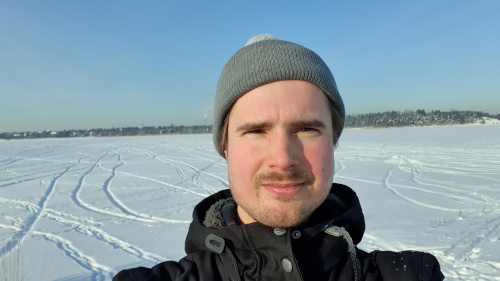
\includegraphics[width=\linewidth]{me1.jpg}
  \caption{Me in my beloved home town Helsinki in the middle of summer (well, technically in Espoo, Otaniemi)}
\end{figure}

\subsection{Education}
\begin{itemize}
\item 2016 Bachelor of Science University of Helsinki\\
\item 2018 Master of Philosophy University of Helsinki
\end{itemize}
\subsection{Research}

\begin{itemize}
\item Downlink Coverage and Rate Analysis of Low Earth Orbit Satellite Constellations Using Stochastic Geometry
  Okati, N., Riihonen, T., Korpi, D., Angervuori, I. Wichman, R., Aug 2020, In : IEEE Transactions on Communications. 68, 8, p. 5120-5134 9079921.\\
\item A. Yastrebova et al., "Theoretical and Simulation-based Analysis of Terrestrial Interference to LEO Satellite Uplinks," GLOBECOM 2020 - 2020 IEEE Global Communications Conference, Taipei, Taiwan, 2020, pp. 1-6, doi: 10.1109/GLOBECOM42002.2020.9347980.
\end{itemize}


\section{Blog posts 2021}
General thoughts on mathematics and engineering, practical instructions and artistic non sense. The themes of this blog are much inspired by challenges encountered in my professional life.

\subsubsection{January – Poisson Process on a Sphere}
Poisson process has a generalization in a large category of manifolds. Particularly Poisson point process on a sphere is useful. Nicely enough, Poisson process on a sphere is equivalent to process in a two dimensional area $ A = [-\pi,\pi] \times [-1,1]$ through the area preserving mapping from $A$ to surface of a sphere
\begin{equation}
  (x,y) \mapsto (r,x,\sin(y)) \nonumber.
\end{equation}


Resulting process interpreted in geographical coordinates $(r,\theta,\varphi)$ is a Poisson point process on a sphere of radius $r$.  Following codes returns a scatter plot of Poisson points on the unit sphere.



GNU/Octave or Matlab:
\begin{verbatim}
%Plot random points on a unit sphere. Returns the points in a vector ref in cartesian coordinates
function refc = poissononsphere(density)
  yMin = -1; yMax = 1;
  xMin=-pi; xMax = pi;
  
  xDelta=xMax-xMin;yDelta=yMax-yMin; %Rectangle dimensions
  numbPoints=poissrnd(density);    %Number of points in the area is a Poisson variable of intensity given as density
  x=xDelta*(rand(numbPoints,1))+xMin;    %Pick points from uniform distribution
  y=yDelta*(rand(numbPoints,1))+yMin;    %Map referencepoints to geographical coordinates
  ref = [x y]';

  refs = [x'; asin(y)'];%Map geographical coordinates to Cartesian coordinates on a unit circle
  r = 1;
  refc = [r*sin(refs(2,:)+pi/2).*cos(refs(1,:)+pi);...
          r*sin(refs(2,:)+pi/2).*sin(refs(1,:)+pi);...
          r*cos(refs(2,:)+pi/2)];

  figure(1)    %Plot
  [X, Y, Z] = sphere;
  surf(X,Y,Z,'EdgeColor','none','FaceColor','black');
  hold on
  scatter3(refc(1,:),refc(2,:),refc(3,:),10,...
           'MarkerFaceColor','yellow',...
           'MarkerEdgeColor','red');
  axis equal
end
\end{verbatim}

Python:

\begin{verbatim}
import numpy as np
import scipy.stats
import matplotlib.pyplot as plt
from mpl_toolkits.mplot3d import axes3d

#Rectangle dimension
xMin=-np.pi;xMax=np.pi;
yMin=-1;yMax=1;
xDelta=xMax-xMin;yDelta=yMax-yMin; #rectangle dimensions

#Density parameter of the Poisson point process. Mean number of points on the sphere
lambda0=1000; 

#Simulate Poisson point process

#Number of point in the area is a Poisson variable of intensity lambda0
numbPoints = scipy.stats.poisson( lambda0 ).rvs()
x = xDelta*scipy.stats.uniform.rvs(0,1,((numbPoints,1)))+xMin
y = yDelta*scipy.stats.uniform.rvs(0,1,((numbPoints,1)))+yMin

#Transform to geographical coordinates
x = x
y = np.arcsin(y)
#Plotting
fig = plt.figure()
ax = plt.axes(projection="3d")
ax.scatter(np.sin(y+np.pi/2)*np.cos(x+np.pi),np.sin(y+np.pi/2)*np.sin(x+np.pi),np.cos(y+np.pi/2), color='r' )
plt.show()
  
\end{verbatim}

Wolfram Language:
\begin{verbatim}
(*lambda is the mean number of points on the unit sphere*) 
  poissononsphere[lambda_] := 
  Module[{nrofpoints, phi, theta, radius, refc, polarp}, 
   nrofpoints = RandomVariate[PoissonDistribution[lambda]];
   polarp = 
    Table[{RandomVariate[UniformDistribution[{-Pi, Pi}]], 
      ArcSin[RandomVariate[UniformDistribution[{-1, 1}]]]}, 
     nrofpoints];
   radius = 1;
   refc = 
    Table[{radius*Sin[polarp[[i]][[2]] + Pi/2]*
       Cos[polarp[[i]][[1]] + Pi],
      radius*Sin[polarp[[i]][[2]] + Pi/2]*Sin[polarp[[i]][[1]] + Pi],
      radius*Cos[polarp[[i]][[2]] + Pi/2]}, {i, nrofpoints}];
   refc
   ];
   ListPointPlot3D[poissononsphere[500], BoxRatios -> {1, 1, 1}]  
\end{verbatim}

\begin{figure}
  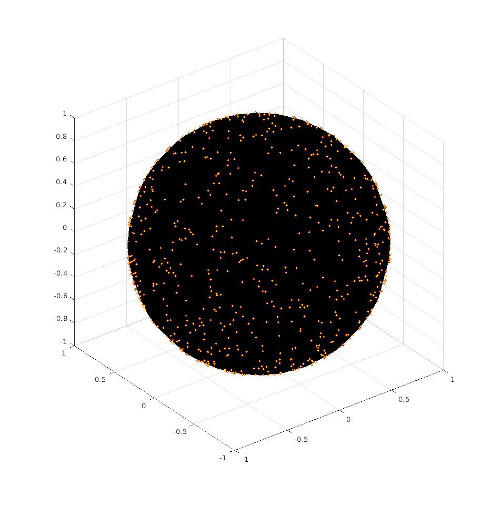
\includegraphics[width=\linewidth]{poissononsphere.jpg}
  \caption{Are the stars Poisson distributed in the sky?}
\end{figure}

\begin{figure}
  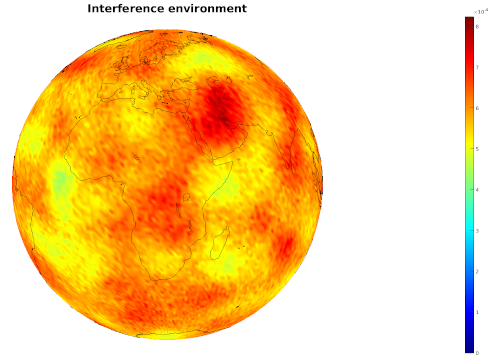
\includegraphics[width=\linewidth]{interferenceenvironment.png}
  \caption{Poisson distributed transmitters and the aggregate signal strength in a satellite by location. Poisson assumption is reasonable in varying situations, but, well, here the sea areas are a bit overrepresented.  }
\end{figure}

References:
\bibitem{theoryofpoint} D. J. Daley and D. Vere-Jones, The General Poisson Process in  ``An introduction to the theory of point processes''. New York: Springer, 2003, pp. 39. 
\bibitem{2} Stoyan, Dietrich. et al. ``Stochastic Geometry and Its Applications''. 3rd ed. Chichester: Wiley, 2013. Print.




\subsection{February – Controlling your Passwords with Pass}
Pass is a nice unix style free and open source wallet for keeping your passwords safe. Here is a brief look how to set it up in Ubuntu.

\begin{itemize}
\item Install the application in the terminal \\
\begin{verbatim}
sudo apt install pass  
\end{verbatim}
\item Check for existing GPG keys \\
\begin{verbatim}
gpg --list-keys 
\end{verbatim}
\item If no keys were found generate a key pair \\
\begin{verbatim}
gpg --generate-key
\end{verbatim}
\item Copy the name of the key and initialize pass\\
\begin{verbatim}
pass init ABCDEFGHIJKLMNOPQRSTUV1234, 
\end{verbatim}
where ABCDEFGHIJKLMNOPQRSTUV1234 is the name of the key.
\item Generate a password with \\
\begin{verbatim}
pass generate keyfolder/newkey 
\end{verbatim}
List passwords
\begin{verbatim}
pass
\end{verbatim}
Copy a password to clipboard \\
\begin{verbatim}
pass keyfolder/newkey -c
\end{verbatim}
For more commands
\begin{verbatim}
man pass
\end{verbatim}
\end{itemize}

Connect pass to git so it is easy to keep track of changes with multiple machines.

\begin{itemize}
\item Export your public and private key to a file with \\
  \begin{verbatim}
gpg --export --output public.key ABCDEFGHIJKLMNOPQRSTUV1234 
gpg --export-secret-key --output private.key ABCDEFGHIJKLMNOPQRSTUV1234,
  \end{verbatim}
  where ABCDEFGHIJKLMNOPQRSTUV1234 is your key name.\\
\item Now we can initialize the git repository with these keys. Move public.key and private.key through a safe channel to a computer you wish to use pass in. Import the keys to the machine \\
\begin{verbatim}
gpg --import public.key
gpg --import private.key
\end{verbatim}
\item After importing keys to a new machine you can initialize pass
\begin{verbatim}
pass init ABCDEFGHIJKLMNOPQRSTUV1234
\end{verbatim}

\item Initialize your git repository. Make a new repository named pass-store e.g. to GitHub if you are doing this first time before the following commands\\
\begin{verbatim}
pass git init 
pass git remote add origin git@repo.com:myname/pass-store
 \end{verbatim}
\item Get password data from the server (from a non-empty repository, otherwise skip)
\begin{verbatim}
pass git pull origin master --allow-unrelated-histories
pass git commit -am "firstcommit"
\end{verbatim}
\item Do some changes and pass will automatically commit them. Push and set upstream \\
\begin{verbatim}
pass git push --set-upstream origin master 
\end{verbatim}
\item From here on you can use the familiar git commands \\
\begin{verbatim}
pass git pull 
pass git push 
\end{verbatim}
\end{itemize}
Stay safe :)


References:

\bibitem[1]{pass}\htmladdnormallink{Password Store}{\pass}


  \subsection{March – Signal Propagation in a City}
Signal propagation in a city is characterized essentially by obstacles which reflects the signal. In a city signal power levels follows approximately \htmladdnormallink{Rayleigh}{\ray} statistics if there is no line-of-sight path present between the transmitter and the receiver. 

Here is just couple of nice figures I made to help myself to perceive what is going on. First figure demonstrates how a single signal propagates between buildings, and second figure shows how aggregate signal power (interference) from many transmitters develops in time. 

  \begin{figure}
  \includegraphics[width=\linewidth]{sin.gif}
  \caption{\htmladdnormallink{Helmholtz equation}{https://en.wikipedia.org/wiki/Helmholtz_equation} solved by \htmladdnormallink{finite element method}{https://en.wikipedia.org/wiki/Finite_element_method}. The white boxes represents buildings, and the little white circle is the transmitter. You can see how reflections will cause the signal strength either to increase or decrease depending on the location.}
\end{figure}


  
  \begin{figure}
  \includegraphics[width=\linewidth]{rician.gif}
  \caption{Interference field developing in time. Transmitters in random locations are moving to random directions in time, and the aggregate signal strength is plotted. There is a line-of-sight component is present – that is we assume in fact  \htmladdnormallink{Rician fading}{\ric}. Red occurrences will cause remarkable disturbance in communication as interference from other transmitters gets large. Time can't be considered to be in scale here.}
\end{figure}


  References:

\bibitem[1]{hurr}François Baccelli, Bartlomiej Blaszczyszyn \htmladdnormallink{Stochastic Geometry and Wireless Networks, Volume I -Theory}{\hal}

  \bibitem[2]{hur22r} Nicolae Cindea (2021).   \htmladdnormallink{Movie to GIF Converter}{https://www.mathworks.com/matlabcentral/fileexchange/17463-movie-to-gif-converter)}, MATLAB Central File Exchange. Retrieved June 14, 2021. 

    

  \subsection{April – Frequentist Inference in Mathematica}
  Mathematica provides a package called ``Hypothesis Testing'' for analyzing random data. Package includes handy objects like ``Around'' which represents a quantity and the uncertainty around it. The following example code returns an Around object representing the $90 \%$ confidence interval of the estimated bias of a coin after a repeated trial. Like shown in the code, the ListPlot plots Around objects as such.


\begin{verbatim}
(*Load the Hypothesis Testing Package.*)
Needs["HypothesisTesting`"];

coin[flips_, bias_] :=
 (*Make the experiment and collect the data*) 
 Module[{index, realizations, mean, conf, around},
  realizations = {};
  For[index = 1, index <= flips, index++,
   realizations =  
     Append[realizations, 
      RandomVariate[BernoulliDistribution[bias]]];
   ];
  
  (*Mean*)
  mean = Mean[realizations[[All]]];
  (*Confidence interval*)
  conf = MeanCI[realizations[[All]]];
  (*Around object*)
  around = Around[mean, Abs[conf[[1]] - conf[[2]]]]
  ]
around = coin[1000, 0.5]
ListPlot[{around}]
\end{verbatim}


\subsection{May – Rayleigh Fading Audiolized}

When a signal is propagating through multiple paths each signal component in each path will be in different phase and of different strength when received. Should there be no line-of-sight component present, the  additive signal will fade according to the \htmladdnormallink{Rayleigh fading}{\ray}.

For example, a simple sine wave

can after some multi-path propagation sound something like

assuming that the receiver is moving at a constant speed, so that variation in multi-path sources Doppler shift will cause the aggregate signal to vary randomly in time.

If we add some \htmladdnormallink{Gaussian white noise}{\gaus}

we notice that the original signal is somehow recognisable from the noise


but the faded signal


will sometimes bury completely under the noise – these events are referred to as \textbf{deep fades}.


Here is a GNU/Octave or Matlab code for the used Rayleigh simulator:
\begin{verbatim}
%Rayleigh simulator. Jakes model. In Octave remember to load the statistics package.

close all
clear all

tic

N = 20; %Number multipaths.
T= linspace(0,10000,100000); %Time.
v = 0.001; %Speed of the receiver.
randan = pi*rand(1,N); %Random angles w.r.t. receiver.
rI = 1000*rand(1,N); %Random distances of the sources.

%Geometrical stuff. Check for the Jakes model in the reference.
An = @(t) (atan(sin(randan).*rI./(cos(randan).*rI-v*t))).*(cos(randan).*rI>v*t)+...
     (pi-atan(sin(randan).*rI./(v*t-cos(randan).*rI))).*(cos(randan).*rI<=v*t);
phis = 2*pi.*(rand(1,N));
wc =pi/2; %Frequency of the signal.
Beta = 2*pi/(1/(wc/(2*pi)));
theta = @(t) cos(An(t)).*Beta*v.*t+phis;

powers = rand(1,N); %Random powers of the signals in the multipaths.
powers = powers./sum(powers); %Normalize the powers.
Ez = @(t) sum(powers.*cos(wc*t+theta(t)));
EZ = []; %Faded signal.
REF = []; %Original signal.
NOISE = []; %Additional Gaussian noise.
for t =T
    EZ = [EZ Ez(t)];
    REF = [REF cos(wc*t)];
    NOISE = [NOISE 0.9*stdnormal_rnd(1)];
end

%Write the audio files at sampling rate 8000.
audiowrite('EZ.wav',EZ,8000)
audiowrite('EZNOISE.wav',1/2*(EZ+NOISE),8000)
audiowrite('REFNOISE.wav', 1/2*(REF+NOISE), 8000)


toc
plot(T,EZ)
\end{verbatim}


And the same in Python:

\begin{verbatim}
import numpy as np
import math
import matplotlib.pyplot as plt
import sounddevice as sd
import time

#Jakes Rayleigh simulator. Please check for the reference in this site for further details.

N = 20 #Number of multipaths.
T = np.linspace(0, 10000, 100000) #Time vector.
v = 0.001 #Speed of the receiver. 



randan = np.random.rand(1, N) * math.pi #Random angles w.r.t. receiver.
rI = np.random.rand(1, N) * 1000 #Random distances of the sources.
phis = np.random.rand(1, N) * 2 * math.pi 

def An(t):
    return (np.arctan(np.sin(randan) * rI / (np.cos(randan) * rI - v * t))) * (
        np.cos(randan) * rI > v * t
    ) + (np.pi - np.arctan(np.sin(randan) * rI / (v * t - np.cos(randan) * rI))) * (
        np.cos(randan) * rI <= v * t
    )

wc = np.pi/2 #Frequency of the signal.
Beta = 2 * math.pi / (1 / (wc / (2 * math.pi)))

def theta(t):
    return np.cos(An(t)) * Beta * v * t +phis

powers = np.random.rand(1,N)*2 #Random powers of the signals in the multipaths.
powers = powers/np.sum(powers) #Normalize powers..

def Ez(t):
    return np.sum(powers * np.cos(wc * t + theta(t)))

EZ = np.vectorize(Ez)(T)
REF = np.vectorize(lambda time : 2*np.cos(wc * time))(T)

#Play and plot.
fs = 8000
sd.play(EZ,fs,blocking = True)
#sd.play(REF,fs,blocking = True)
plt.plot(T, EZ)
plt.show()  
\end{verbatim}



References:
\bibitem[1]{theoryofpoint} William C. Jakes, ``Microwave Mobile Communications'', IEEE PRESS, 1974. 



  \subsection{June – MIMO}
  Multiple-input and multiple-output (\htmladdnormallink{MIMO}{https://en.wikipedia.org/wiki/MIMO}) antenna technology is used to exploit the \htmladdnormallink{multi-path propagation}{\ray} to improve the capacity of a communication link (i.e. more gigabytes of internet speed). In principle, capacity can always be increased merely by increasing the power of the transmitting antenna. However – apart from being energy consuming – this increases also interference to any other receivers should they operate in the same frequency band. In MIMO the energy is divided among multiple antennas, and the link capacity is improved without using any extra energy and without increasing the interference to other transmitters.

  But how and why does it work? Here is how I came up with a simple argument based on stochastic geometry.

  Let us make few assumptions. We assume a flat and infinite Earth (no tin-foils). In addition we assume that our communication channel environment consists of many obstacles so that our transmitting antenna and receiving antenna cant see each other. We can assume that we are in a city full of houses, cars, trees, etc.. Then our data signal is prone to propagate to the receiver through multiple paths; for example through different streets around different houses. Aggregate signal in the receiver will be \htmladdnormallink{Rayleigh faded}{\ray}. City is full of mobile phones transmitting data with their base-stations, and in the other hand causing interference to each other. We make a natural assumption that the interfering transmitters are distributed according to the \htmladdnormallink{Poisson point process}{https://en.wikipedia.org/wiki/Poisson_point_process}.


  As derived in \htmladdnormallink{here}{\hall} we express the probability $p$ of a successful transmission (for example a message to a friend) as:

  \begin{equation*}
    \mathbb{P}[\text{Message received}] = e^{-\frac{\pi^2}{2\sqrt{P}}},
  \end{equation*}
  
  where $P$ denotes the mean transmitting power.

  In MIMO we use multiple antennas to send the message. In each antenna the message should be coded in a way that it can't be mixed with the information that the other antennas are transmitting. This can be done by \htmladdnormallink{orthogonal modulation}{https://en.wikipedia.org/wiki/Orthogonal_frequency_division_multiplexing}.
  Assuming that each message from each antenna will propagate to the receiver in an independent way, we can calculate by complementary probability that at least one message is received:
  
  \begin{equation*}
    \mathbb{P}[\text{Message received}]  = 1-\left(1-e^{-\frac{\pi^2}{2\sqrt{P/N}}}\right)^N,
  \end{equation*}
  
where $N$ is the number of antennas. Notice that we divided the transmitting power $P$ by number of antennas, so we don't increase the aggregate power at all.
In the other hand, should we have no MIMO technology at hand, we could try to improve to increase the link quality just by increasing the power $P$. In the following figure we compare these two cases.

  \begin{figure}
  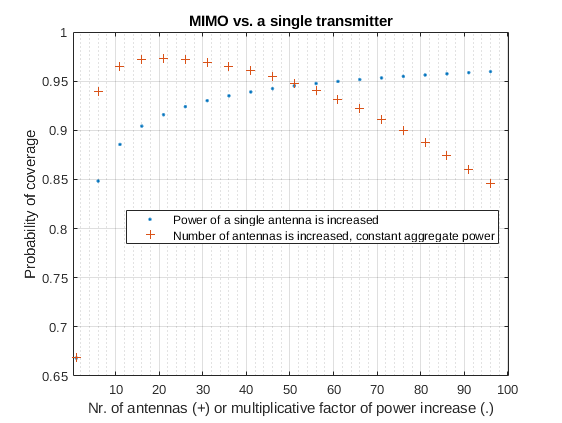
\includegraphics[width=\linewidth]{MIMO.png}
  \caption{MIMO saves energy and improves the quality}
  \end{figure}

  It is evident that MIMO is a great solution for increasing the throughput of a wireless communication link. Using MIMO we can achieve better data-rates than by increasing the power of the transmitters.

  \bibitem[1]{hal2}François Baccelli, Bartlomiej Blaszczyszyn \htmladdnormallink{Stochastic Geometry and Wireless Networks, Volume 2 - Applications}{\hall}
   
\end{document}
%
% optional post-title formatting for PostScript
%
\parindent0pt
\parskip2.5ex plus 0.5ex minus 0.5ex

